\section{Questionnaires}

We conducted a questionnaire with the aim of verifying, on a large scale,
the needs that were found in the interviews.\\
The questionnaire was structured to make it possible to select a completion
language (i.e. English or Italian), and then to navigate among its sections.
The choice of the dual language stems from the idea of wanting to reach as
many people as possible in order to validate the observations relating to the
interview phase, with an important consequence: as the sample size increases,
the audience considered tends to be more heterogeneous, that is,
it becomes less likely to consider only a particular target.\\
In fact, the questionnaire reached a larger audience than that
considered in the interview phase, reaching over 160 people.\\
We present below the most interesting considerations that resulted
from the questionnaires:\\

\begin{itemize}
    \item Only 12\% of interviewed people claim that they never order takeway food
    (the remaining 88\% do it at least sometimes).
    \item About 58\% of them find it convenient so that they do not have to cook. 50\%
    claim that it is fast and they can save time.
    \item The majority of people either order via phone call or use a general food ordering
    app.
    \item Almost three quarters of interviewed people  would use a voice chatbot to make
    a food order. Almost 80\% of them think that it would be easy and fast to use. More
    than a quarter of them is a technology enthusiast, and would just use for the
    sake of it.
    \item The most frequent reasons that the remaining quarter of people that would not
    use such a system have are: the impossibility to visually check a menu and the need
    of an app to do that; less comfortable experience; wariness for voice assistants.
\end{itemize}


\subsection{Meaningful charts}

\begin{figure}[h]
    \centering
    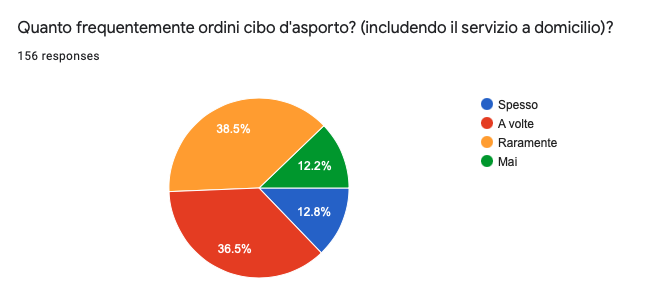
\includegraphics[scale=0.5]{images/q_freq.png}
    \caption{Takeaway order frequency.}
    \label{fig:q_freq}
\end{figure}

\begin{figure}[h]
    \centering
    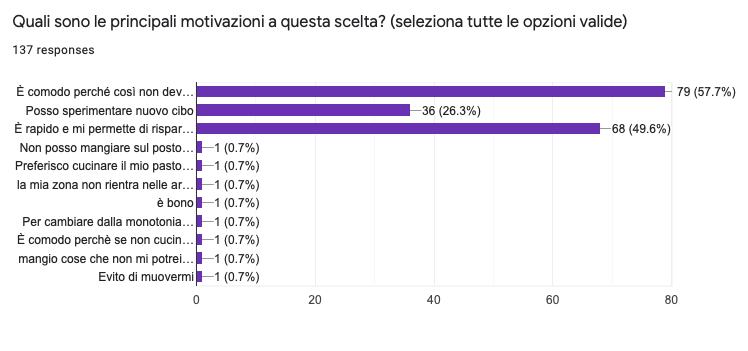
\includegraphics[scale=0.5]{images/q_r1.png}
    \caption{Reasons for ordering takeaway food.}
    \label{fig:q_r1}
\end{figure}

\begin{figure}[h]
    \centering
    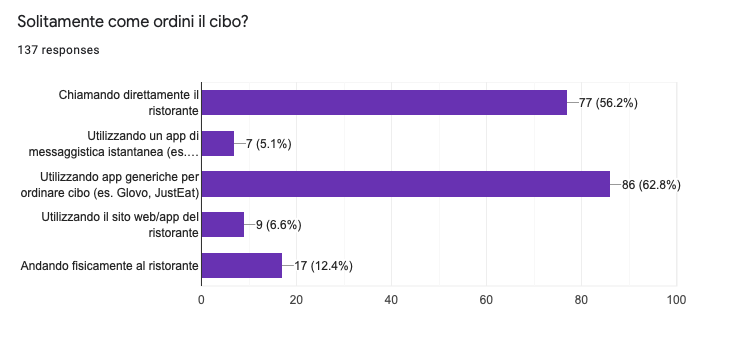
\includegraphics[scale=0.5]{images/q_h.png}
    \caption{Ways of ordering takeaway food.}
    \label{fig:q_h}
\end{figure}

\begin{figure}[h]
    \centering
    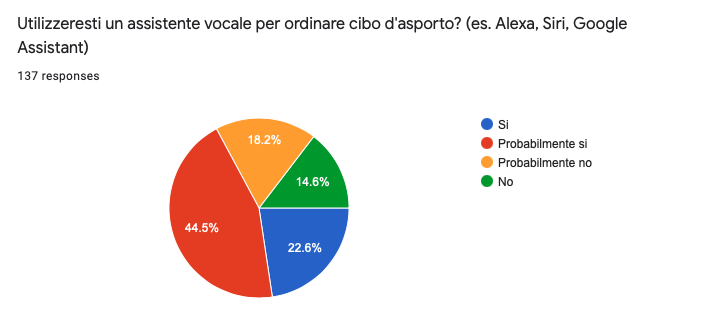
\includegraphics[scale=0.5]{images/q_v.png}
    \caption{Opionions on using a voice chatbot for ordering food.}
    \label{fig:q_v}
\end{figure}

\begin{figure}[h]
    \centering
    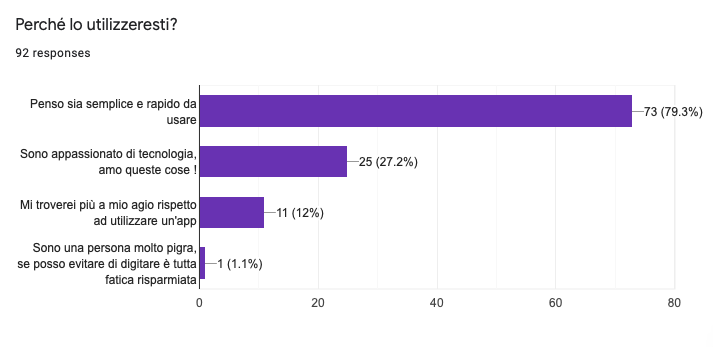
\includegraphics[scale=0.5]{images/q_r2.png}
    \caption{Reasons to use a voice chatbot to order food.}
    \label{fig:q_r2}
\end{figure}